\chapter{Практическая часть}

\section{Формат входных данных}

Входные данные содержатся в папке "Data/Input/". Файл "WholeMesh.txt" содержит данные о трёхмерной сетке, из которой автоматически строится сетка для решения двумерной задачи на нормальном поле. В файле содержится информация о границах расчётной  области по $x$, $y$, $z$, количество необходимых разбиений для каждой оси, коэффициенты разрядки, количество областей с разными значениями удельной электропроводности и информация о границах расчётной области. Полностью формат изображен на рисунке \ref{fig:TextWholeMesh}.

\begin{figure}
	\centering
	\vspace*{0.7cm}
	\includegraphics[width=0.8\linewidth]{images/"inputMeshText".png}
	\caption{Входной формат сетки по пространству}
	\label{fig:TextWholeMesh}
\end{figure}

Входные данные для учёта поля влияния хранятся в папке "Data/Input/Anomalies/". Каждый файл, находящийся в этой папке, содержит примерно похожий формат хранения, как и для основной сетки. Задаются границы по осям $x$, $y$, $z$, количество необходимых разбиений для каждой оси, коэффициенты разрядки, значения удельной электропроводности на аномальной области и границы этой области. Полностью формат изображен на рисунке \ref{fig:TextAnomalyMesh}.

\begin{figure}
	\centering
	\vspace*{0.7cm}
	\includegraphics[width=0.8\linewidth]{images/"inputAnomalyText".png}
	\caption{Входной формат сетки по пространству для аномалии}
	\label{fig:TextAnomalyMesh}
\end{figure}

Входные данные для сетки по времени, содержатся в файле "Time.txt", в папке "Data/Input/" и содержат четыре значения: время начала и конца, количество разбиений и коэффициент разрядки.

\section{Сборка глобальной матрицы и глобального вектора правой части}

При формировании матрицы \textbf{A} для решения СЛАУ необходимо учитывать соответствие локальной к глобальной нумерации каждого узла. Глобальная нумерация узлов сетки однозначно определяет вклад локальной матрицы в соответствующие строчки и столбцы матрицы \textbf{A}. Поэтому, зная глобальную нумерацию узлов конечного элемента, можно определить какие элементы глобальной матрицы изменятся при добавлении в нее локальной. Аналогичным образом определяется вклад локального вектора правой части в глобальный.

\section{Учёт краевых условий}

Поскольку в решаемой задаче у нас на всех границах задаётся однородное краевое условие первого рода, технически необходимо в соответствующей строчке матрицы обнулить вне диагональные элементы, на диагонали поставить значение 1, а в соответствующую строчку вектора правой части поставить значение краевого условия на этой границе, т.е. в нашем случае тоже обнулить.

\section{Решение СЛАУ}

Для решения СЛАУ мы будем использовать локально-оптимальную схему c ILU-предобусловливанием \cite{9}. Это хороший и быстрый метод решения систем уравнений для несимметричных матриц. Перед решением СЛАУ задаются параметры для досрочного выхода из итерационного процесса, а именно: выход по максимальному количеству совершённых итераций и минимальному значению нормы вектора невязки.

В результате решения СЛАУ мы получим вектор $q$ весов базисных функций, на которые раскладывается функция $A_{\varphi}^0$ или вектор-функция $\overrightarrow{\textbf{A}}^{+}$. Учитывая построение базисных функций, компонентами этого вектора будут значения функции в соответствующих узлах сетки.

\section{Определение значения вектор-потенциала и напряжённости электрического поля}

После решения СЛАУ вида (\ref{eq_2_27}) или (\ref{eq_2_43}), необходимо найти напряжённость электрического поля по формуле (\ref{eq_2_28}). Пользуясь аналитическим представлением из (\ref{eq_2_23}), программная реализация будет выглядеть следующим образом.

Поскольку в качестве конечных элементов использовались прямоугольники для двумерной и прямые параллелепипеды для трёхмерной задач, то можно упростить алгоритм нахождения значения функции на элементе. Можно не перебирать каждый элемент отдельно и проверять значение интересующей точки на принадлежность ему, а последовательно сравнивать координаты точки со значениями на разбиениях по осям координат. Тогда сложность алгоритма будет не $O(n^2)$ для двумерной или $O(n^3)$ для трёхмерной задач, а $O(k \cdot n)$, где $n$ -- количество отрезков, на которые разбиваются оси координат.

\section{Тестирование двумерной задачи на полиномах}

Проведем сначала тестирование программы на работоспособность для уравнения (\ref{eq_4_1}). В таблицах \ref{tab:test2D1} -- \ref{tab:test2D9} представлен результат тестирования на полиномиальных функциях. Образец расчетной области изображен на рисунке \ref{fig:exampleOf3DMesh}. Это область $\Omega = [1.0, 2.0]_r \times [1.0, 2.0]_z$, она содержит 16 узлов, а на всех границах будем задавать первые краевые условия. 

\begin{equation} \label{eq_4_1}
	-\frac{1}{r} \frac{\partial}{\partial r} \left(r \frac{\partial u}{\partial r}\right) - \frac{\partial^2 u}{\partial z^2} + \frac{u}{r^2} + \sigma \frac{\partial u}{\partial t} = f,
\end{equation}

\begin{figure}
	\centering
	\vspace*{0.7cm}
	\includegraphics[width=0.75\linewidth]{images/"TestMesh".png}
	\caption{Расчетная область}
	\label{fig:exampleOf3DMesh}
\end{figure}

\begin{table}
	\caption{Тестирование при $u = 2$, $f = \frac{2}{r^2}$, $\sigma = 0$}
	\centering
	\small
	\begin{tabularx}{1.0\textwidth}{| >{\raggedright\arraybackslash}X | >{\raggedright\arraybackslash}X | >{\raggedright\arraybackslash}X |>{\raggedright\arraybackslash}X |}
		\hline
		\centering{Узел} & \centering{Значение} & \centering{Абсолютная погрешность} & \centering{Относительная погрешность} \tabularnewline \hline
		
		
		
		\centering{(${}^4/_3$; ${}^4/_3$)} & \centering{2.00226896E+000}& \centering{2.26896083E-003} & \centering{1.13448042E-003} \tabularnewline \hline
		
		\centering{(${}^5/_3$; ${}^4/_3$)} & \centering{2.00130487E+000} & \centering{1.30486533E-003} & \centering{6.52432666E-004} \tabularnewline \hline
		
		\centering{(${}^4/_3$; ${}^5/_3$)} & \centering{2.00226896E+000} & \centering{2.26896083E-003} & \centering{1.13448042E-003} \tabularnewline \hline
		
		\centering{(${}^5/_3$; ${}^5/_3$)} & \centering{2.00130487E+000} & \centering{1.30486533E-003} & \centering{6.52432666E-004} \tabularnewline \hline
		
	\end{tabularx}
	\label{tab:test2D1}
\end{table}

\begin{table}
	\caption{Тестирование при $u = r$, $f = 0$, $\sigma = 0$}
	\centering
	\small
	\begin{tabularx}{1.0\textwidth}{| >{\raggedright\arraybackslash}X | >{\raggedright\arraybackslash}X | >{\raggedright\arraybackslash}X |>{\raggedright\arraybackslash}X |}
		\hline
		\centering{Узел} & \centering{Значение} & \centering{Абсолютная погрешность} & \centering{Относительная погрешность} \tabularnewline \hline
		
		
		
		\centering{(${}^4/_3$; ${}^4/_3$)} & \centering{1.33333333E+000}& \centering{1.33226763E-015} & \centering{9.99200722E-016} \tabularnewline \hline
		
		\centering{(${}^5/_3$; ${}^4/_3$)} & \centering{1.66666667E+000} & \centering{6.66133815E-016} & \centering{3.99680289E-016} \tabularnewline \hline
		
		\centering{(${}^4/_3$; ${}^5/_3$)} & \centering{1.33333333E+000} & \centering{1.77635684E-015} & \centering{1.33226763E-015} \tabularnewline \hline
		
		\centering{(${}^5/_3$; ${}^5/_3$)} & \centering{1.66666667E+000} & \centering{6.66133815E-016} & \centering{3.99680289E-016} \tabularnewline \hline
		
	\end{tabularx}
	\label{tab:test2D2}
\end{table}

\begin{table}
	\caption{Тестирование при $u = z$, $f = \frac{z}{r^2}$, $\sigma = 0$}
	\centering
	\small
	\begin{tabularx}{1.0\textwidth}{| >{\raggedright\arraybackslash}X | >{\raggedright\arraybackslash}X | >{\raggedright\arraybackslash}X |>{\raggedright\arraybackslash}X |}
		\hline
		\centering{Узел} & \centering{Значение} & \centering{Абсолютная погрешность} & \centering{Относительная погрешность} \tabularnewline \hline
		
		
		
		\centering{(${}^4/_3$; ${}^4/_3$)} & \centering{1.33491362E+000}& \centering{1.58028263E-003} & \centering{1.18521198E-003} \tabularnewline \hline
		
		\centering{(${}^5/_3$; ${}^4/_3$)} & \centering{1.33426439E+000} & \centering{9.31054340E-004} & \centering{6.98290755E-004} \tabularnewline \hline
		
		\centering{(${}^4/_3$; ${}^5/_3$)} & \centering{1.66848983E+000} & \centering{1.82315862E-003} & \centering{1.09389517E-003} \tabularnewline \hline
		
		\centering{(${}^5/_3$; ${}^5/_3$)} & \centering{1.66769291E+000} & \centering{1.02624366E-003} & \centering{6.15746195E-004} \tabularnewline \hline
		
	\end{tabularx}
	\label{tab:test2D3}
\end{table}

\begin{table}
	\caption{Тестирование при $u = r+z$, $f = \frac{z}{r^2}$, $\sigma = 0$}
	\centering
	\small
	\begin{tabularx}{1.0\textwidth}{| >{\raggedright\arraybackslash}X | >{\raggedright\arraybackslash}X | >{\raggedright\arraybackslash}X |>{\raggedright\arraybackslash}X |}
		\hline
		\centering{Узел} & \centering{Значение} & \centering{Абсолютная погрешность} & \centering{Относительная погрешность} \tabularnewline \hline
		
		
		
		\centering{(${}^4/_3$; ${}^4/_3$)} & \centering{2.66824695E+000}& \centering{1.58028263E-003} & \centering{5.92605988E-004} \tabularnewline \hline
		
		\centering{(${}^5/_3$; ${}^4/_3$)} & \centering{3.00093105E+000} & \centering{9.31054340E-004} & \centering{3.10351447E-004} \tabularnewline \hline
		
		\centering{(${}^4/_3$; ${}^5/_3$)} & \centering{3.00182316E+000} & \centering{1.82315862E-003} & \centering{6.07719539E-004} \tabularnewline \hline
		
		\centering{(${}^5/_3$; ${}^5/_3$)} & \centering{3.33435958E+000} & \centering{1.02624366E-003} & \centering{3.07873097E-004} \tabularnewline \hline
		
	\end{tabularx}
	\label{tab:test2D4}
\end{table}

\begin{table}
	\caption{Тестирование при $u = rz$, $f = 0$, $\sigma = 0$}
	\centering
	\small
	\begin{tabularx}{1.0\textwidth}{| >{\raggedright\arraybackslash}X | >{\raggedright\arraybackslash}X | >{\raggedright\arraybackslash}X |>{\raggedright\arraybackslash}X |}
		\hline
		\centering{Узел} & \centering{Значение} & \centering{Абсолютная погрешность} & \centering{Относительная погрешность} \tabularnewline \hline
		
		
		
		\centering{(${}^4/_3$; ${}^4/_3$)} & \centering{1.77777778E+000}& \centering{1.11022302E-015} & \centering{6.24500451E-016} \tabularnewline \hline
		
		\centering{(${}^5/_3$; ${}^4/_3$)} & \centering{2.22222222E+000} & \centering{3.10862447E-015} & \centering{1.39888101E-015} \tabularnewline \hline
		
		\centering{(${}^4/_3$; ${}^5/_3$)} & \centering{2.22222222E+000} & \centering{8.88178420E-016} & \centering{3.99680289E-016} \tabularnewline \hline
		
		\centering{(${}^5/_3$; ${}^5/_3$)} & \centering{2.77777778E+000} & \centering{4.88498131E-015} & \centering{1.75859327E-015} \tabularnewline \hline
		
	\end{tabularx}
	\label{tab:test2D5}
\end{table}

\begin{table}
	\caption{Тестирование при $u = r^2 + z^2$, $f = \frac{z^2}{r^2} - 5$, $\sigma = 0$}
	\centering
	\small
	\begin{tabularx}{1.0\textwidth}{| >{\raggedright\arraybackslash}X | >{\raggedright\arraybackslash}X | >{\raggedright\arraybackslash}X |>{\raggedright\arraybackslash}X |}
		\hline
		\centering{Узел} & \centering{Значение} & \centering{Абсолютная погрешность} & \centering{Относительная погрешность} \tabularnewline \hline
		
		
		
		\centering{(${}^4/_3$; ${}^4/_3$)} & \centering{3.55717205E+000}& \centering{1.61649660E-003} & \centering{4.54639669E-004} \tabularnewline \hline
		
		\centering{(${}^5/_3$; ${}^4/_3$)} & \centering{4.55644336E+000} & \centering{8.87803368E-004} & \centering{1.94883666E-004} \tabularnewline \hline
		
		\centering{(${}^4/_3$; ${}^5/_3$)} & \centering{4.55790068E+000} & \centering{2.34512455E-003} & \centering{5.14783438E-004} \tabularnewline \hline
		
		\centering{(${}^5/_3$; ${}^5/_3$)} & \centering{5.55672893E+000} & \centering{1.17337132E-003} & \centering{2.11206838E-004} \tabularnewline \hline
		
	\end{tabularx}
	\label{tab:test2D6}
\end{table}

\begin{table}
	\caption{Тестирование при $u = r^2 z^2$, $f = -3z^2 - 2r^2$, $\sigma = 0$}
	\centering
	\small
	\begin{tabularx}{1.0\textwidth}{| >{\raggedright\arraybackslash}X | >{\raggedright\arraybackslash}X | >{\raggedright\arraybackslash}X |>{\raggedright\arraybackslash}X |}
		\hline
		\centering{Узел} & \centering{Значение} & \centering{Абсолютная погрешность} & \centering{Относительная погрешность} \tabularnewline \hline
		
		
		
		\centering{(${}^4/_3$; ${}^4/_3$)} & \centering{3.15919390E+000}& \centering{1.29993140E-003} & \centering{4.11306418E-004} \tabularnewline \hline
		
		\centering{(${}^5/_3$; ${}^4/_3$)} & \centering{4.93728492E+000} & \centering{9.86688136E-004} & \centering{1.99804348E-004} \tabularnewline \hline
		
		\centering{(${}^4/_3$; ${}^5/_3$)} & \centering{4.93658403E+000} & \centering{1.68757555E-003} & \centering{3.41734049E-004} \tabularnewline \hline
		
		\centering{(${}^5/_3$; ${}^5/_3$)} & \centering{7.71481536E+000} & \centering{1.23402231E-003} & \centering{1.59929291E-004} \tabularnewline \hline
		
	\end{tabularx}
	\label{tab:test2D7}
\end{table}

\begin{table}
	\caption{Тестирование при $u = r^3+z^3$, $f = -8r -6z + \frac{z^3}{r^2}$, $\sigma = 0$}
	\centering
	\small
	\begin{tabularx}{1.0\textwidth}{| >{\raggedright\arraybackslash}X | >{\raggedright\arraybackslash}X | >{\raggedright\arraybackslash}X |>{\raggedright\arraybackslash}X |}
		\hline
		\centering{Узел} & \centering{Значение} & \centering{Абсолютная погрешность} & \centering{Относительная погрешность} \tabularnewline \hline
		
		
		
		\centering{(${}^4/_3$; ${}^4/_3$)} & \centering{4.73874864E+000}& \centering{1.99210278E-003} & \centering{4.20209180E-004} \tabularnewline \hline
		
		\centering{(${}^5/_3$; ${}^4/_3$)} & \centering{6.99757994E+000} & \centering{2.42006018E-003} & \centering{3.45722883E-004} \tabularnewline \hline
		
		\centering{(${}^4/_3$; ${}^5/_3$)} & \centering{6.99968104E+000} & \centering{3.18957115E-004} & \centering{4.55653022E-005} \tabularnewline \hline
		
		\centering{(${}^5/_3$; ${}^5/_3$)} & \centering{9.25749495E+000} & \centering{1.76431155E-003} & \centering{1.90545647E-004} \tabularnewline \hline
		
	\end{tabularx}
	\label{tab:test2D8}
\end{table}

\begin{table}
	\caption{Тестирование при $u = r^3 z^3$, $f = -8rz^3 - 6r^3 z$, $\sigma = 0$}
	\centering
	\small
	\begin{tabularx}{1.0\textwidth}{| >{\raggedright\arraybackslash}X | >{\raggedright\arraybackslash}X | >{\raggedright\arraybackslash}X |>{\raggedright\arraybackslash}X |}
		\hline
		\centering{Узел} & \centering{Значение} & \centering{Абсолютная погрешность} & \centering{Относительная погрешность} \tabularnewline \hline
		
		
		
		\centering{(${}^4/_3$; ${}^4/_3$)} & \centering{5.60268110E+000}& \centering{1.59745896E-002} & \centering{2.84313374E-003} \tabularnewline \hline
		
		\centering{(${}^5/_3$; ${}^4/_3$)} & \centering{1.09603120E+001} & \centering{1.36249123E-002} & \centering{1.24157014E-003} \tabularnewline \hline
		
		\centering{(${}^4/_3$; ${}^5/_3$)} & \centering{1.09509327E+001} & \centering{2.30042146E-002} & \centering{2.09625906E-003} \tabularnewline \hline
		
		\centering{(${}^5/_3$; ${}^5/_3$)} & \centering{2.14142095E+001} & \centering{1.92609735E-002} & \centering{8.98639979E-004} \tabularnewline \hline
		
	\end{tabularx}
	\label{tab:test2D9}
\end{table}

Исходя из полученных данных, можно сказать, что программа верно находит численное решение задачи.

Рассмотрим решение функции $u = e^{r \cdot z}$, последовательно разбивая сетку в 2 раза. Результаты тестирования приведены в таблице \ref{tab:test2D10}.

\begin{table}
	\caption{Тестирование при $u = e^{r \cdot z}$, $\sigma = 0$}
	\centering
	\small
	\begin{tabularx}{1.0\textwidth}{| >{\raggedright\arraybackslash}X | >{\raggedright\arraybackslash}X | >{\raggedright\arraybackslash}X |>{\raggedright\arraybackslash}X |}
		\hline
		\centering{Количество разбиений} & \centering{Средняя погрешность} & \centering{$\text{log}_2\left(\frac{\sigma_{i-1}}{\sigma_i}\right)$} \tabularnewline \hline		
		
		\centering{2} & \centering{1.7116567E-004}& \centering{-} \tabularnewline \hline
		
		\centering{4} & \centering{5.2066366E-005} & \centering{1.716969754} \tabularnewline \hline
		
		\centering{8} & \centering{1.4089198E-005} & \centering{1.885762274} \tabularnewline \hline
		
		\centering{16} & \centering{3.6602112E-006} & \centering{1.94459064} \tabularnewline \hline
		
		\centering{32} & \centering{9.3301457E-007} & \centering{1.971955381} \tabularnewline \hline
		
	\end{tabularx}
	\label{tab:test2D10}
\end{table}

Порядок сходимости стремится к 2.

Теперь проведём тестирование уравнения (\ref{eq_4_1}) на порядок аппроксимации и сходимости для аппроксимации по времени. Для чистоты исследования мы не будем учитывать слагаемое с ${}^1/_{r^2}$. Сетка по времени равномерная $t \in [0, 1]$, $h_t = 0.2$. При тестировании на порядок сходимости будем рассматривать функцию $u = e^t$ и $f = e^t$. Результат тестирования представлен в таблице \ref{tab:test2D11}.

\begin{table}
	\caption{Тестирование при $u = e^t$, $f = e^t$}
	\centering
	\small
	\begin{tabularx}{1.0\textwidth}{| >{\raggedright\arraybackslash}X | >{\raggedright\arraybackslash}X | >{\raggedright\arraybackslash}X |>{\raggedright\arraybackslash}X |}
		\hline
		\centering{Количество разбиений} & \centering{Средняя погрешность} & \centering{$\text{log}_2\left(\frac{\sigma_{i-1}}{\sigma_i}\right)$} \tabularnewline \hline		
		
		\centering{4} & \centering{8.4940866E-003} & \centering{-} \tabularnewline \hline
		
		\centering{8} & \centering{2.4848144E-003} & \centering{1.77332095} \tabularnewline \hline
		
		\centering{16} & \centering{6.6533732E-004} & \centering{1.90098023} \tabularnewline \hline
		
		\centering{32} & \centering{1.7191414E-004} & \centering{1.95239775} \tabularnewline \hline
		
	\end{tabularx}
	\label{tab:test2D11}
\end{table}

Порядок сходимости стремится к 2.

Поскольку мы использовали трёхслойную неявную схему, то для тестирования на порядок аппроксимации рассмотрим функцию $u = t^2$, и $f = 2 \cdot t$. Результат  тестирования представлен в таблице \ref{tab:test2D12}.

\begin{table}
	\caption{Тестирование при $u = t^2$, $f = 2 \cdot t$, $\sigma = 1$}
	\centering
	\small
	\begin{tabularx}{1.0\textwidth}{| >{\raggedright\arraybackslash}X | >{\raggedright\arraybackslash}X |>{\raggedright\arraybackslash}X |}
		\hline
		\centering{Временной слой} & \centering{Абсолютная погрешность} & \centering{Относительная погрешность} \tabularnewline \hline
		
		\centering{0.0} & \centering{0.0000000E+000 \\ 0.0000000E+000 \\ 
		0.0000000E+000 \\ 
		0.0000000E+000} & \centering{- \\ - \\ - \\ -} \tabularnewline \hline
		
		\centering{0.2} & \centering{0.0000000E+000 \\ 0.0000000E+000 \\ 
			0.0000000E+000 \\ 
			0.0000000E+000} & \centering{0.0000000E+000 \\ 0.0000000E+000 \\ 
			0.0000000E+000 \\ 
			0.0000000E+000} \tabularnewline \hline
		
		\centering{0.4} & \centering{8.3266727E-017 \\
			2.7755576E-017 \\
			2.7755576E-017 \\
			8.3266727E-017} & \centering{5.2041704E-016 \\
			1.7347235E-016 \\
			1.7347235E-016 \\
			5.2041704E-016} \tabularnewline \hline
		
		\centering{0.6} & \centering{5.5511151E-017 \\
			5.5511151E-017 \\
			5.5511151E-017 \\
			5.5511151E-017} & \centering{1.5419764E-016 \\
			1.5419764E-016 \\
			1.5419764E-016 \\
			1.5419764E-016} \tabularnewline \hline
		
		\centering{0.8} & \centering{5.5511151E-016 \\
			0.0000000E+000 \\
			1.1102230E-016 \\
			2.2204460E-016} & \centering{8.6736174E-016 \\
			0.0000000E+000 \\ 
			1.7347235E-016 \\ 
			3.4694470E-016} \tabularnewline \hline
		
		\centering{1.0} & \centering{4.4408921E-016 \\
			0.0000000E+000
			0.0000000E+000
			4.4408921E-016} & \centering{4.4408921E-016 \\
			0.0000000E+000 \\
			0.0000000E+000 \\
			4.4408921E-016} \tabularnewline \hline
		
	\end{tabularx}
	\label{tab:test2D12}
\end{table}

Как и предполагалось, квадратичная функция по времени находится без численной погрешности.

\section{Тестирование трёхмерной задачи на полиномиальных вектор-функциях}

Проведем сначала тестирование разработанной программы по векторному МКЭ на работоспособность. Образец расчетной области изображен на рисунке \ref{fig:exampleOfArea}. Это область $\Omega = [0.0, 3.0]_x \times [0.0, 3.0]_y \times [0.0, 3.0]_z$, она содержит 144 ребра, на всех границах будем задавать первые краевые условия. 

\begin{figure}
	\centering
	\vspace*{0.7cm}
	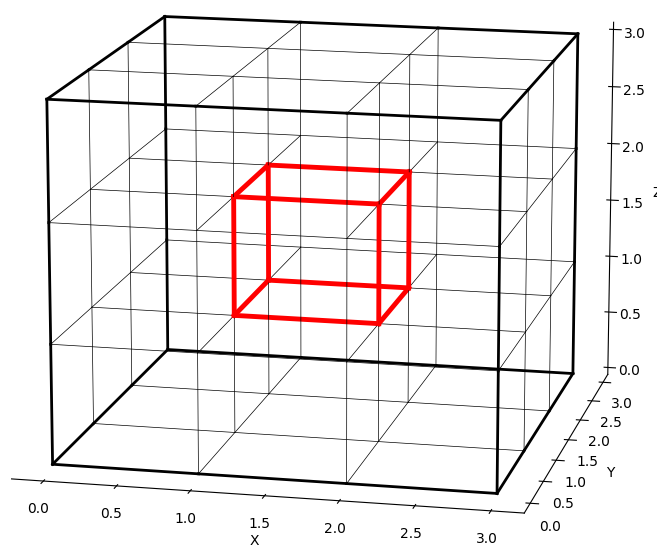
\includegraphics[width=0.7\linewidth]{images/3D_grid_example.png}
	\caption{Расчетная область}
	\label{fig:exampleOfArea}
\end{figure}

Тестирование будем проводить дифференциального уравнения (\ref{eq_4_2}):

\begin{equation} \label{eq_4_2}
	\text{rot} \left(\frac{1}{\mu} \text{rot} \overrightarrow{\textbf{A}}\right) + \gamma \overrightarrow{\textbf{A}} + \sigma \frac{\partial \overrightarrow{\textbf{A}}}{\partial t} = \overrightarrow{\textbf{F}}.
\end{equation}

В таблицах \ref{tab:test1} -- \ref{tab:test9} приведено тестирование на работоспособность программы. Для искомых $\overrightarrow{\textbf{A}}$ будем выводить значения функции в центрах рёбер сетки, отмеченных красным цветом на рисунке \ref{fig:exampleOfArea}.

\begin{table}
	\caption{Тестирование при $\overrightarrow{\textbf{A}} = (1.0, 1.0, 1.0)^{\text{T}}$, $\overrightarrow{\textbf{F}} = (1.0, 1.0, 1.0)^{\text{T}}$, $\mu = 1$, $\gamma = 1$, $\sigma = 0$}
	\centering
	\small
	\begin{tabularx}{1.0\textwidth}{| >{\raggedright\arraybackslash}X | >{\raggedright\arraybackslash}X | >{\raggedright\arraybackslash}X |>{\raggedright\arraybackslash}X |}
		\hline
		\centering{Ребро} & \centering{Значение} & \centering{Абсолютная погрешность} & \centering{Относительная погрешность} \tabularnewline \hline
		
		
		\centering{($x; 1.0; 1.0$)} & \centering{1.00000000E+000}& \centering{0.00000000E+000} & \centering{0.00000000E+000} \tabularnewline \hline
		
		\centering{($x; 2.0; 1.0$)} & \centering{1.00000000E+000}& \centering{0.00000000E+000} & \centering{0.00000000E+000} \tabularnewline \hline
		
		\centering{($x; 1.0; 2.0$)} & \centering{1.00000000E+000}& \centering{0.00000000E+000} & \centering{0.00000000E+000} \tabularnewline \hline
		
		\centering{($x; 2.0; 2.0$)} & \centering{1.00000000E+000}& \centering{0.00000000E+000} & \centering{0.00000000E+000} \tabularnewline \hline
		
		
		
		\centering{($1.0; y; 1.0$)} & \centering{1.00000000E+000}& \centering{0.00000000E+000} & \centering{0.00000000E+000} \tabularnewline \hline
		
		\centering{($2.0; y; 1.0$)} & \centering{1.00000000E+000}& \centering{0.00000000E+000} & \centering{0.00000000E+000} \tabularnewline \hline
		
		\centering{($1.0; y; 2.0$)} & \centering{1.00000000E+000}& \centering{0.00000000E+000} & \centering{0.00000000E+000} \tabularnewline \hline
		
		\centering{($2.0; y; 2.0$)} & \centering{1.00000000E+000}& \centering{0.00000000E+000} & \centering{0.00000000E+000} \tabularnewline \hline
		
		
		
		\centering{($1.0; 1.0; z$)} & \centering{1.00000000E+000}& \centering{0.00000000E+000} & \centering{0.00000000E+000} \tabularnewline \hline
		
		\centering{($2.0; 1.0; z$)} & \centering{1.00000000E+000}& \centering{0.00000000E+000} & \centering{0.00000000E+000} \tabularnewline \hline
		
		\centering{($1.0; 2.0; z$)} & \centering{1.00000000E+000}& \centering{0.00000000E+000} & \centering{0.00000000E+000} \tabularnewline \hline
		
		\centering{($2.0; 2.0; z$)} & \centering{1.00000000E+000}& \centering{0.00000000E+000} & \centering{0.00000000E+000} \tabularnewline \hline
		
		
	\end{tabularx}
	\label{tab:test1}
\end{table}

\begin{table}
	\caption{Тестирование при $\overrightarrow{\textbf{A}} = (y, z, x)^{\text{T}}$, $\overrightarrow{\textbf{F}} = (y, z, x)^{\text{T}}$, $\mu = 1$, $\gamma = 1$, $\sigma = 0$}
	\centering
	\small
	\begin{tabularx}{1.0\textwidth}{| >{\raggedright\arraybackslash}X | >{\raggedright\arraybackslash}X | >{\raggedright\arraybackslash}X |>{\raggedright\arraybackslash}X |}
		\hline
		\centering{Ребро} & \centering{Значение} & \centering{Абсолютная погрешность} & \centering{Относительная погрешность} \tabularnewline \hline
		
		\centering{($x; 1.0; 1.0$)} & \centering{1.00000000E+000}& \centering{0.00000000E+000} & \centering{0.00000000E+000} \tabularnewline \hline
		
		\centering{($x; 2.0; 1.0$)} & \centering{2.00000000E+000}& \centering{0.00000000E+000} & \centering{0.00000000E+000} \tabularnewline \hline
		
		\centering{($x; 1.0; 2.0$)} & \centering{1.00000000E+000}& \centering{0.00000000E+000} & \centering{0.00000000E+000} \tabularnewline \hline
		
		\centering{($x; 2.0; 2.0$)} & \centering{2.00000000E+000}& \centering{0.00000000E+000} & \centering{0.00000000E+000} \tabularnewline \hline
		
		
		
		\centering{($1.0; y; 1.0$)} & \centering{1.00000000E+000}& \centering{0.00000000E+000} & \centering{0.00000000E+000} \tabularnewline \hline
		
		\centering{($2.0; y; 1.0$)} & \centering{1.00000000E+000}& \centering{0.00000000E+000} & \centering{0.00000000E+000} \tabularnewline \hline
		
		\centering{($1.0; y; 2.0$)} & \centering{2.00000000E+000}& \centering{0.00000000E+000} & \centering{0.00000000E+000} \tabularnewline \hline
		
		\centering{($2.0; y; 2.0$)} & \centering{2.00000000E+000}& \centering{0.00000000E+000} & \centering{0.00000000E+000} \tabularnewline \hline
		
		
		
		\centering{($1.0; 1.0; z$)} & \centering{1.00000000E+000}& \centering{0.00000000E+000} & \centering{0.00000000E+000} \tabularnewline \hline
		
		\centering{($2.0; 1.0; z$)} & \centering{2.00000000E+000}& \centering{0.00000000E+000} & \centering{0.00000000E+000} \tabularnewline \hline
		
		\centering{($1.0; 2.0; z$)} & \centering{1.00000000E+000}& \centering{0.00000000E+000} & \centering{0.00000000E+000} \tabularnewline \hline
		
		\centering{($2.0; 2.0; z$)} & \centering{2.00000000E+000}& \centering{0.00000000E+000} & \centering{0.00000000E+000} \tabularnewline \hline
		
		
	\end{tabularx}
	\label{tab:test2}
\end{table}

\begin{table}
	\caption{Тестирование при $\overrightarrow{\textbf{A}} = (1 + y + x; 1 + x + z; 1 + x + y)^{\text{T}}$, $\overrightarrow{\textbf{F}} = (1 + y + x; 1 + x + z; 1 + x + y)^{\text{T}}$, $\mu = 1$, $\gamma = 1$, $\sigma = 0$}
	\centering
	\small
	\begin{tabularx}{1.0\textwidth}{| >{\raggedright\arraybackslash}X | >{\raggedright\arraybackslash}X | >{\raggedright\arraybackslash}X |>{\raggedright\arraybackslash}X |}
		\hline
		\centering{Ребро} & \centering{Значение} & \centering{Абсолютная погрешность} & \centering{Относительная погрешность} \tabularnewline \hline
		
		
		\centering{($x; 1.0; 1.0$)} & \centering{3.00000000E+000}& \centering{0.00000000E+000} & \centering{0.00000000E+000} \tabularnewline \hline
		
		\centering{($x; 2.0; 1.0$)} & \centering{4.00000000E+000}& \centering{0.00000000E+000} & \centering{0.00000000E+000} \tabularnewline \hline
		
		\centering{($x; 1.0; 2.0$)} & \centering{4.00000000E+000}& \centering{0.00000000E+000} & \centering{0.00000000E+000} \tabularnewline \hline
		
		\centering{($x; 2.0; 2.0$)} & \centering{5.00000000E+000}& \centering{0.00000000E+000} & \centering{0.00000000E+000} \tabularnewline \hline
		
		
		
		\centering{($1.0; y; 1.0$)} & \centering{3.00000000E+000}& \centering{0.00000000E+000} & \centering{0.00000000E+000} \tabularnewline \hline
		
		\centering{($2.0; y; 1.0$)} & \centering{4.00000000E+000}& \centering{0.00000000E+000} & \centering{0.00000000E+000} \tabularnewline \hline
		
		\centering{($1.0; y; 2.0$)} & \centering{4.00000000E+000}& \centering{0.00000000E+000} & \centering{0.00000000E+000} \tabularnewline \hline
		
		\centering{($2.0; y; 2.0$)} & \centering{5.00000000E+000}& \centering{0.00000000E+000} & \centering{0.00000000E+000} \tabularnewline \hline
		
		
		
		\centering{($1.0; 1.0; z$)} & \centering{3.00000000E+000}& \centering{0.00000000E+000} & \centering{0.00000000E+000} \tabularnewline \hline
		
		\centering{($2.0; 1.0; z$)} & \centering{4.00000000E+000}& \centering{0.00000000E+000} & \centering{0.00000000E+000} \tabularnewline \hline
		
		\centering{($1.0; 2.0; z$)} & \centering{4.00000000E+000}& \centering{0.00000000E+000} & \centering{0.00000000E+000} \tabularnewline \hline
		
		\centering{($2.0; 2.0; z$)} & \centering{5.00000000E+000}& \centering{0.00000000E+000} & \centering{0.00000000E+000} \tabularnewline \hline
		
	\end{tabularx}
	\label{tab:test3}
\end{table}

\begin{table}
	\caption{Тестирование при $\overrightarrow{\textbf{A}} = (y - z; x - z; x - y)^{\text{T}}$, $\overrightarrow{\textbf{F}} = (y - x; x - z; x - y)^{\text{T}}$, $\mu = 1$, $\gamma = 1$, $\sigma = 0$}
	\centering
	\small
	\begin{tabularx}{1.0\textwidth}{| >{\raggedright\arraybackslash}X | >{\raggedright\arraybackslash}X | >{\raggedright\arraybackslash}X |>{\raggedright\arraybackslash}X |}
		\hline
		\centering{Ребро} & \centering{Значение} & \centering{Абсолютная погрешность} & \centering{Относительная погрешность} \tabularnewline \hline
		
		
		\centering{($x; 1.0; 1.0$)} & \centering{2.35132600E-016}& \centering{2.35132600E-016} & \centering{0.00000000E+000} \tabularnewline \hline
		
		\centering{($x; 2.0; 1.0$)} & \centering{1.00000000E+000}& \centering{0.00000000E+000} & \centering{0.00000000E+000} \tabularnewline \hline
		
		\centering{($x; 1.0; 2.0$)} & \centering{-1.00000000E+000}& \centering{0.00000000E+000} & \centering{0.00000000E+000} \tabularnewline \hline
		
		\centering{($x; 2.0; 2.0$)} & \centering{-5.55111512E-016}& \centering{-5.55111512E-016} & \centering{0.00000000E+000} \tabularnewline \hline
		
		
		
		\centering{($1.0; y; 1.0$)} & \centering{-3.97378607E-016}& \centering{-3.97378607E-016} & \centering{0.00000000E+000} \tabularnewline \hline
		
		\centering{($2.0; y; 1.0$)} & \centering{1.00000000E+000}& \centering{0.00000000E+000} & \centering{0.00000000E+000} \tabularnewline \hline
		
		\centering{($1.0; y; 2.0$)} & \centering{-1.00000000E+000}& \centering{0.00000000E+000} & \centering{0.00000000E+000} \tabularnewline \hline
		
		\centering{($2.0; y; 2.0$)} & \centering{-1.94289029E-016}& \centering{-1.94289029E-016} & \centering{0.00000000E+000} \tabularnewline \hline
		
		
		
		\centering{($1.0; 1.0; z$)} & \centering{-2.74847895E-016}& \centering{-2.74847895E-016} & \centering{0.00000000E+000} \tabularnewline \hline
		
		\centering{($2.0; 1.0; z$)} & \centering{1.00000000E+000}& \centering{0.00000000E+000} & \centering{0.00000000E+000} \tabularnewline \hline
		
		\centering{($1.0; 2.0; z$)} & \centering{-1.00000000E+000}& \centering{0.00000000E+000} & \centering{0.00000000E+000} \tabularnewline \hline
		
		\centering{($2.0; 2.0; z$)} & \centering{4.27842044E-016}& \centering{4.27842044E-016} & \centering{0.00000000E+000} \tabularnewline \hline
		
		
	\end{tabularx}
	\label{tab:test4}
\end{table}

\begin{table}
	\caption{Тестирование при $\overrightarrow{\textbf{A}} = (y \cdot z; x \cdot z; x \cdot y)^{\text{T}}$, $\overrightarrow{\textbf{F}} = (y \cdot z; x \cdot z; x \cdot y)^{\text{T}}$, $\mu = 1$, $\gamma = 1$, $\sigma = 0$}
	\centering
	\small
	\begin{tabularx}{1.0\textwidth}{| >{\raggedright\arraybackslash}X | >{\raggedright\arraybackslash}X | >{\raggedright\arraybackslash}X |>{\raggedright\arraybackslash}X |}
		\hline
		\centering{Ребро} & \centering{Значение} & \centering{Абсолютная погрешность} & \centering{Относительная погрешность} \tabularnewline \hline
		
		
		\centering{($x; 1.0; 1.0$)} & \centering{1.00000000E+000}& \centering{0.00000000E+000} & \centering{0.00000000E+000} \tabularnewline \hline
		
		\centering{($x; 2.0; 1.0$)} & \centering{2.00000000E+000}& \centering{0.00000000E+000} & \centering{0.00000000E+000} \tabularnewline \hline
		
		\centering{($x; 1.0; 2.0$)} & \centering{2.00000000E+000}& \centering{0.00000000E+000} & \centering{0.00000000E+000} \tabularnewline \hline
		
		\centering{($x; 2.0; 2.0$)} & \centering{4.00000000E+000}& \centering{0.00000000E+000} & \centering{0.00000000E+000} \tabularnewline \hline
		
		
		
		\centering{($1.0; y; 1.0$)} & \centering{1.00000000E+000}& \centering{0.00000000E+000} & \centering{0.00000000E+000} \tabularnewline \hline
		
		\centering{($2.0; y; 1.0$)} & \centering{2.00000000E+000}& \centering{0.00000000E+000} & \centering{0.00000000E+000} \tabularnewline \hline
		
		\centering{($1.0; y; 2.0$)} & \centering{2.00000000E+000}& \centering{0.00000000E+000} & \centering{0.00000000E+000} \tabularnewline \hline
		
		\centering{($2.0; y; 2.0$)} & \centering{4.00000000E+000}& \centering{0.00000000E+000} & \centering{0.00000000E+000} \tabularnewline \hline
		
		\centering{($1.0; 1.0; z$)} & \centering{1.00000000E+000}& \centering{0.00000000E+000} & \centering{0.00000000E+000} \tabularnewline \hline
		
		\centering{($2.0; 1.0; z$)} & \centering{2.00000000E+000}& \centering{0.00000000E+000} & \centering{0.00000000E+000} \tabularnewline \hline
		
		\centering{($1.0; 2.0; z$)} & \centering{2.00000000E+000}& \centering{0.00000000E+000} & \centering{0.00000000E+000} \tabularnewline \hline
		
		\centering{($2.0; 2.0; z$)} & \centering{4.00000000E+000}& \centering{0.00000000E+000} & \centering{0.00000000E+000} \tabularnewline \hline
		
	\end{tabularx}
	\label{tab:test5}
\end{table}

\begin{table}
	\caption{Тестирование при $\overrightarrow{\textbf{A}} = (y^2; z^2; x^2)^{\text{T}}$, $\overrightarrow{\textbf{F}} = (y^2 - 2; z^2 - 2; x^2 - 2)^{\text{T}}$, $\mu = 1$, $\gamma = 1$, $\sigma = 0$}
	\centering
	\small
	\begin{tabularx}{1.0\textwidth}{| >{\raggedright\arraybackslash}X | >{\raggedright\arraybackslash}X | >{\raggedright\arraybackslash}X |>{\raggedright\arraybackslash}X |}
		\hline
		\centering{Ребро} & \centering{Значение} & \centering{Абсолютная погрешность} & \centering{Относительная погрешность} \tabularnewline \hline
		
		
		\centering{($x; 1.0; 1.0$)} & \centering{1.00000000E+000}& \centering{0.00000000E+000} & \centering{0.00000000E+000} \tabularnewline \hline
		
		\centering{($x; 2.0; 1.0$)} & \centering{4.00000000E+000}& \centering{0.00000000E+000} & \centering{0.00000000E+000} \tabularnewline \hline
		
		\centering{($x; 1.0; 2.0$)} & \centering{1.00000000E+000}& \centering{0.00000000E+000} & \centering{0.00000000E+000} \tabularnewline \hline
		
		\centering{($x; 2.0; 2.0$)} & \centering{4.00000000E+000}& \centering{0.00000000E+000} & \centering{0.00000000E+000} \tabularnewline \hline
		
		
		
		\centering{($1.0; y; 1.0$)} & \centering{1.00000000E+000}& \centering{0.00000000E+000} & \centering{0.00000000E+000} \tabularnewline \hline
		
		\centering{($2.0; y; 1.0$)} & \centering{1.00000000E+000}& \centering{0.00000000E+000} & \centering{0.00000000E+000} \tabularnewline \hline
		
		\centering{($1.0; y; 2.0$)} & \centering{4.00000000E+000}& \centering{0.00000000E+000} & \centering{0.00000000E+000} \tabularnewline \hline
		
		\centering{($2.0; y; 2.0$)} & \centering{4.00000000E+000}& \centering{0.00000000E+000} & \centering{0.00000000E+000} \tabularnewline \hline
		
		
		
		\centering{($1.0; 1.0; z$)} & \centering{1.00000000E+000}& \centering{0.00000000E+000} & \centering{0.00000000E+000} \tabularnewline \hline
		
		\centering{($2.0; 1.0; z$)} & \centering{4.00000000E+000}& \centering{0.00000000E+000} & \centering{0.00000000E+000} \tabularnewline \hline
		
		\centering{($1.0; 2.0; z$)} & \centering{1.00000000E+000}& \centering{0.00000000E+000} & \centering{0.00000000E+000} \tabularnewline \hline
		
		\centering{($2.0; 2.0; z$)} & \centering{4.00000000E+000}& \centering{0.00000000E+000} & \centering{0.00000000E+000} \tabularnewline \hline
	\end{tabularx}
	\label{tab:test6}
\end{table}

\begin{table}
	\caption{Тестирование при $\overrightarrow{\textbf{A}} = (y^2 + z^2; x^2 + z^2; x^2 + y^2)^{\text{T}}$, $\overrightarrow{\textbf{F}} = (y^2 + z^2 - 4; x^2 + z^2 - 4; x^2 + y^2 - 4)^{\text{T}}$, $\mu = 1$, $\gamma = 1$, $\sigma = 0$}
	\centering
	\small
	\begin{tabularx}{1.0\textwidth}{| >{\raggedright\arraybackslash}X | >{\raggedright\arraybackslash}X | >{\raggedright\arraybackslash}X |>{\raggedright\arraybackslash}X |}
		\hline
		\centering{Ребро} & \centering{Значение} & \centering{Абсолютная погрешность} & \centering{Относительная погрешность} \tabularnewline \hline
		
		
		\centering{($x; 1.0; 1.0$)} & \centering{2.00000000E+000}& \centering{0.00000000E+000} & \centering{0.00000000E+000} \tabularnewline \hline
		
		\centering{($x; 2.0; 1.0$)} & \centering{5.00000000E+000}& \centering{0.00000000E+000} & \centering{0.00000000E+000} \tabularnewline \hline
		
		\centering{($x; 1.0; 2.0$)} & \centering{5.00000000E+000}& \centering{0.00000000E+000} & \centering{0.00000000E+000} \tabularnewline \hline
		
		\centering{($x; 2.0; 2.0$)} & \centering{8.00000000E+000}& \centering{0.00000000E+000} & \centering{0.00000000E+000} \tabularnewline \hline
		
		
		
		\centering{($1.0; y; 1.0$)} & \centering{2.00000000E+000}& \centering{0.00000000E+000} & \centering{0.00000000E+000} \tabularnewline \hline
		
		\centering{($2.0; y; 1.0$)} & \centering{5.00000000E+000}& \centering{0.00000000E+000} & \centering{0.00000000E+000} \tabularnewline \hline
		
		\centering{($1.0; y; 2.0$)} & \centering{5.00000000E+000}& \centering{0.00000000E+000} & \centering{0.00000000E+000} \tabularnewline \hline
		
		\centering{($2.0; y; 2.0$)} & \centering{8.00000000E+000}& \centering{0.00000000E+000} & \centering{0.00000000E+000} \tabularnewline \hline
		
		
		
		\centering{($1.0; 1.0; z$)} & \centering{2.00000000E+000}& \centering{0.00000000E+000} & \centering{0.00000000E+000} \tabularnewline \hline
		
		\centering{($2.0; 1.0; z$)} & \centering{5.00000000E+000}& \centering{0.00000000E+000} & \centering{0.00000000E+000} \tabularnewline \hline
		
		\centering{($1.0; 2.0; z$)} & \centering{5.00000000E+000}& \centering{0.00000000E+000} & \centering{0.00000000E+000} \tabularnewline \hline
		
		\centering{($2.0; 2.0; z$)} & \centering{8.00000000E+000}& \centering{0.00000000E+000} & \centering{0.00000000E+000} \tabularnewline \hline
		
	\end{tabularx}
	\label{tab:test7}
\end{table}

\begin{table}
	\caption{Тестирование при $\overrightarrow{\textbf{A}} = (y^3; 0; 0)^{\text{T}}$, $\overrightarrow{\textbf{F}} = (y^3 - 6y; 0; 0)^{\text{T}}$, $\mu = 1$, $\gamma = 1$, $\sigma = 0$}
	\centering
	\small
	\begin{tabularx}{1.0\textwidth}{| >{\raggedright\arraybackslash}X | >{\raggedright\arraybackslash}X | >{\raggedright\arraybackslash}X |>{\raggedright\arraybackslash}X |}
		\hline
		\centering{Ребро} & \centering{Значение} & \centering{Абсолютная погрешность} & \centering{Относительная погрешность} \tabularnewline \hline
		
		
		\centering{($x; 1.0; 1.0$)} & \centering{1.00000000E+000}& \centering{0.00000000E+000} & \centering{0.00000000E+000} \tabularnewline \hline
		
		\centering{($x; 2.0; 1.0$)} & \centering{8.00000000E+000}& \centering{0.00000000E+000} & \centering{0.00000000E+000} \tabularnewline \hline
		
		\centering{($x; 1.0; 2.0$)} & \centering{1.00000000E+000}& \centering{0.00000000E+000} & \centering{0.00000000E+000} \tabularnewline \hline
		
		\centering{($x; 2.0; 2.0$)} & \centering{8.00000000E+000}& \centering{0.00000000E+000} & \centering{0.00000000E+000} \tabularnewline \hline
		
		
		
		\centering{($1.0; y; 1.0$)} & \centering{0.00000000E+000}& \centering{0.00000000E+000} & \centering{0.00000000E+000} \tabularnewline \hline
		
		\centering{($2.0; y; 1.0$)} & \centering{0.00000000E+000}& \centering{0.00000000E+000} & \centering{0.00000000E+000} \tabularnewline \hline
		
		\centering{($1.0; y; 2.0$)} & \centering{0.00000000E+000}& \centering{0.00000000E+000} & \centering{0.00000000E+000} \tabularnewline \hline
		
		\centering{($2.0; y; 2.0$)} & \centering{0.00000000E+000}& \centering{0.00000000E+000} & \centering{0.00000000E+000} \tabularnewline \hline
		
		
		
		\centering{($1.0; 1.0; z$)} & \centering{0.00000000E+000}& \centering{0.00000000E+000} & \centering{0.00000000E+000} \tabularnewline \hline
		
		\centering{($2.0; 1.0; z$)} & \centering{0.00000000E+000}& \centering{0.00000000E+000} & \centering{0.00000000E+000} \tabularnewline \hline
		
		\centering{($1.0; 2.0; z$)} & \centering{0.00000000E+000}& \centering{0.00000000E+000} & \centering{0.00000000E+000} \tabularnewline \hline
		
		\centering{($2.0; 2.0; z$)} & \centering{0.00000000E+000}& \centering{0.00000000E+000} & \centering{0.00000000E+000} \tabularnewline \hline
		
	\end{tabularx}
	\label{tab:test8}
\end{table}

\begin{table}
	\caption{Тестирование при $\overrightarrow{\textbf{A}} = (y^2 \cdot z^2; x^2 \cdot z^2; x^2 \cdot y^2)^{\text{T}}$, $\overrightarrow{\textbf{F}} = (y^2 \cdot z^2 - 2(y^2 + z^2); x^2 \cdot z^2 - 2(x^2 + z^2); x^2 \cdot y^2 - 2(x^2 + y^2))^{\text{T}}$, $\mu = 1$, $\gamma = 1$, $\sigma = 0$}
	\centering
	\small
	\begin{tabularx}{1.0\textwidth}{| >{\raggedright\arraybackslash}X | >{\raggedright\arraybackslash}X | >{\raggedright\arraybackslash}X |>{\raggedright\arraybackslash}X |}
		\hline
		\centering{Ребро} & \centering{Значение} & \centering{Абсолютная погрешность} & \centering{Относительная погрешность} \tabularnewline \hline
		
		
		\centering{($x; 1.0; 1.0$)} & \centering{1.00000000E+000}& \centering{0.00000000E+000} & \centering{0.00000000E+000} \tabularnewline \hline
		
		\centering{($x; 2.0; 1.0$)} & \centering{4.00000000E+000}& \centering{0.00000000E+000} & \centering{0.00000000E+000} \tabularnewline \hline
		
		\centering{($x; 1.0; 2.0$)} & \centering{4.00000000E+000}& \centering{0.00000000E+000} & \centering{0.00000000E+000} \tabularnewline \hline
		
		\centering{($x; 2.0; 2.0$)} & \centering{1.60000000E+001}& \centering{0.00000000E+000} & \centering{0.00000000E+000} \tabularnewline \hline
		
		
		
		\centering{($1.0; y; 1.0$)} & \centering{1.00000000E+000}& \centering{0.00000000E+000} & \centering{0.00000000E+000} \tabularnewline \hline
		
		\centering{($2.0; y; 1.0$)} & \centering{4.00000000E+000}& \centering{0.00000000E+000} & \centering{0.00000000E+000} \tabularnewline \hline
		
		\centering{($1.0; y; 2.0$)} & \centering{4.00000000E+000}& \centering{0.00000000E+000} & \centering{0.00000000E+000} \tabularnewline \hline
		
		\centering{($2.0; y; 2.0$)} & \centering{1.60000000E+001}& \centering{0.00000000E+000} & \centering{0.00000000E+000} \tabularnewline \hline
		
		
		
		\centering{($1.0; 1.0; z$)} & \centering{1.00000000E+000}& \centering{0.00000000E+000} & \centering{0.00000000E+000} \tabularnewline \hline
		
		\centering{($2.0; 1.0; z$)} & \centering{4.00000000E+000}& \centering{0.00000000E+000} & \centering{0.00000000E+000} \tabularnewline \hline
		
		\centering{($1.0; 2.0; z$)} & \centering{4.00000000E+000}& \centering{0.00000000E+000} & \centering{0.00000000E+000} \tabularnewline \hline
		
		\centering{($2.0; 2.0; z$)} & \centering{1.60000000E+001}& \centering{0.00000000E+000} & \centering{0.00000000E+000} \tabularnewline \hline
		
	\end{tabularx}
	\label{tab:test9}
\end{table}

Проведём тестирование на порядок аппроксимации. Для оценки будем брать значения вектор-функции в центрах параллелепипедов. Сетка по пространству для данных тестов изображена на рисунке \ref{fig:exampleOfArea_1}.

\begin{figure}
	\centering
	\vspace*{0.7cm}
	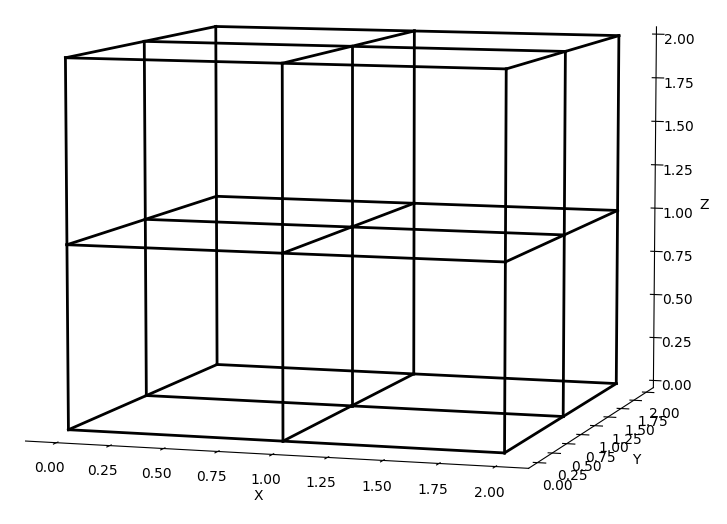
\includegraphics[width=0.5\linewidth]{images/3D_mesh_1.png}
	\caption{Расчетная область}
	\label{fig:exampleOfArea_1}
\end{figure}

В таблицах \ref{tab:test10} -- \ref{tab:test11} представлены результаты тестирования для постоянной и линейной вектор-функциях.

\begin{table}
	\caption{Тестирование при $\overrightarrow{\textbf{A}} = (1.0; 1.0; 1.0)^{\text{T}}$, $\overrightarrow{\textbf{F}} = (1.0; 1.0; 1.0)^{\text{T}}$, $\mu = 1$, $\gamma = 1$, $\sigma = 0$}
	\centering
	\small
	\begin{tabularx}{1.0\textwidth}{| >{\raggedright\arraybackslash}X | >{\raggedright\arraybackslash}X | >{\raggedright\arraybackslash}X |>{\raggedright\arraybackslash}X |}
		\hline
		\centering{Ребро} & \centering{Значение} & \centering{Абсолютная погрешность} & \centering{Относительная погрешность} \tabularnewline \hline
		
		
		\centering{($0.5; 0.5; 0.5$)} & \centering{1.00000000E+000 \\ 1.00000000E+000\\
			1.00000000E+000}& \centering{0.00000000E+000 \\ 0.00000000E+000 \\ 0.00000000E+000} & \centering{0.00000000E+000 \\ 0.00000000E+000 \\ 0.00000000E+000} \tabularnewline \hline
		
		\centering{($1.5; 0.5; 0.5$)} & \centering{1.00000000E+000 \\ 1.00000000E+000\\
			1.00000000E+000}& \centering{0.00000000E+000 \\ 0.00000000E+000 \\ 0.00000000E+000} & \centering{0.00000000E+000 \\ 0.00000000E+000 \\ 0.00000000E+000} \tabularnewline \hline
		
		\centering{($0.5; 1.5; 0.5$)} & \centering{1.00000000E+000 \\ 1.00000000E+000\\
			1.00000000E+000}& \centering{0.00000000E+000 \\ 0.00000000E+000 \\ 0.00000000E+000} & \centering{0.00000000E+000 \\ 0.00000000E+000 \\ 0.00000000E+000} \tabularnewline \hline
		
		\centering{($1.5; 1.5; 0.5$)} & \centering{1.00000000E+000 \\ 1.00000000E+000\\
			1.00000000E+000}& \centering{0.00000000E+000 \\ 0.00000000E+000 \\ 0.00000000E+000} & \centering{0.00000000E+000 \\ 0.00000000E+000 \\ 0.00000000E+000} \tabularnewline \hline
			
		\centering{($0.5; 0.5; 1.5$)} & \centering{1.00000000E+000 \\ 1.00000000E+000\\
			1.00000000E+000}& \centering{0.00000000E+000 \\ 0.00000000E+000 \\ 0.00000000E+000} & \centering{0.00000000E+000 \\ 0.00000000E+000 \\ 0.00000000E+000} \tabularnewline \hline
		
		\centering{($1.5; 0.5; 1.5$)} & \centering{1.00000000E+000 \\ 1.00000000E+000\\
			1.00000000E+000}& \centering{0.00000000E+000 \\ 0.00000000E+000 \\ 0.00000000E+000} & \centering{0.00000000E+000 \\ 0.00000000E+000 \\ 0.00000000E+000} \tabularnewline \hline
		
		\centering{($0.5; 1.5; 1.5$)} & \centering{1.00000000E+000 \\ 1.00000000E+000\\
			1.00000000E+000}& \centering{0.00000000E+000 \\ 0.00000000E+000 \\ 0.00000000E+000} & \centering{0.00000000E+000 \\ 0.00000000E+000 \\ 0.00000000E+000} \tabularnewline \hline
		
		\centering{($1.5; 1.5; 1.5$)} & \centering{1.00000000E+000 \\ 1.00000000E+000\\
			1.00000000E+000}& \centering{0.00000000E+000 \\ 0.00000000E+000 \\ 0.00000000E+000} & \centering{0.00000000E+000 \\ 0.00000000E+000 \\ 0.00000000E+000} \tabularnewline \hline
	
	\end{tabularx}
	\label{tab:test10}
\end{table}

\begin{table}
	\caption{Тестирование при $\overrightarrow{\textbf{A}} = (y; z; x)^{\text{T}}$, $\overrightarrow{\textbf{F}} = (y; z; x)^{\text{T}}$, $\mu = 1$, $\gamma = 1$, $\sigma = 0$}
	\centering
	\small
	\begin{tabularx}{1.0\textwidth}{| >{\raggedright\arraybackslash}X | >{\raggedright\arraybackslash}X | >{\raggedright\arraybackslash}X |>{\raggedright\arraybackslash}X |}
		\hline
		\centering{Ребро} & \centering{Значение} & \centering{Абсолютная погрешность} & \centering{Относительная погрешность} \tabularnewline \hline
		
		
		\centering{($0.5; 0.5; 0.5$)} & \centering{5.00000000E-001 \\ 5.00000000E-001 \\
			5.00000000E-001}& \centering{0.00000000E+000 \\ 0.00000000E+000 \\ 0.00000000E+000} & \centering{0.00000000E+000 \\ 0.00000000E+000 \\ 0.00000000E+000} \tabularnewline \hline
		
		\centering{($1.5; 0.5; 0.5$)} & \centering{5.00000000E-001 \\ 5.00000000E-001\\
			1.50000000E+000}& \centering{0.00000000E+000 \\ 0.00000000E+000 \\ 0.00000000E+000} & \centering{0.00000000E+000 \\ 0.00000000E+000 \\ 0.00000000E+000} \tabularnewline \hline
		
		\centering{($0.5; 1.5; 0.5$)} & \centering{1.50000000E+000 \\ 5.00000000E-001\\
			5.00000000E-001}& \centering{0.00000000E+000 \\ 0.00000000E+000 \\ 0.00000000E+000} & \centering{0.00000000E+000 \\ 0.00000000E+000 \\ 0.00000000E+000} \tabularnewline \hline
		
		\centering{($1.5; 1.5; 0.5$)} & \centering{1.50000000E+000 \\ 5.00000000E-001\\
			1.50000000E+000}& \centering{0.00000000E+000 \\ 0.00000000E+000 \\ 0.00000000E+000} & \centering{0.00000000E+000 \\ 0.00000000E+000 \\ 0.00000000E+000} \tabularnewline \hline
		
		\centering{($0.5; 0.5; 1.5$)} & \centering{5.00000000E-001 \\ 1.50000000E+000\\
			5.00000000E-001}& \centering{0.00000000E+000 \\ 0.00000000E+000 \\ 0.00000000E+000} & \centering{0.00000000E+000 \\ 0.00000000E+000 \\ 0.00000000E+000} \tabularnewline \hline
		
		\centering{($1.5; 0.5; 1.5$)} & \centering{5.00000000E-001 \\ 1.50000000E+000\\
			5.00000000E-001}& \centering{0.00000000E+000 \\ 0.00000000E+000 \\ 0.00000000E+000} & \centering{0.00000000E+000 \\ 0.00000000E+000 \\ 0.00000000E+000} \tabularnewline \hline
		
		\centering{($0.5; 1.5; 1.5$)} & \centering{1.50000000E+000 \\ 1.50000000E+000\\
			5.00000000E-001}& \centering{0.00000000E+000 \\ 0.00000000E+000 \\ 0.00000000E+000} & \centering{0.00000000E+000 \\ 0.00000000E+000 \\ 0.00000000E+000} \tabularnewline \hline
		
		\centering{($1.5; 1.5; 1.5$)} & \centering{1.50000000E+000 \\ 1.50000000E+000\\
			1.50000000E+000}& \centering{0.00000000E+000 \\ 0.00000000E+000 \\ 0.00000000E+000} & \centering{0.00000000E+000 \\ 0.00000000E+000 \\ 0.00000000E+000} \tabularnewline \hline
		
	\end{tabularx}
	\label{tab:test11}
\end{table}

Как и предполагали, при использовании билинейных вектор-функций точное решение находится вплоть до линейной вектор-функции без численной погрешности.

Проведём теперь тестирование на порядок сходимости на сетке изображённой на рисунке \ref{fig:exampleOfArea}. Для этого последовательно будем разбивать сетку в 2 раза сначала по оси $x$, потом по $y$ и затем по $z$. Результаты тестирования приведены в таблицах \ref{tab:test12} -- \ref{tab:test14}.

\begin{table}
	\caption{Тестирование при $\overrightarrow{\textbf{A}} = (0; 0; e^x)^{\text{T}}$, $\overrightarrow{\textbf{F}} = (0; 0; 0)^{\text{T}}$, $\mu = 1$, $\gamma = 1$, $\sigma = 0$}
	\centering
	\small
	\begin{tabularx}{1.0\textwidth}{| >{\raggedright\arraybackslash}X | >{\raggedright\arraybackslash}X | >{\raggedright\arraybackslash}X |>{\raggedright\arraybackslash}X |}
		\hline
		\centering{Шаг по оси $x$} & \centering{Средняя погрешность} & \centering{$\text{log}_2\left(\frac{\sigma_{i-1}}{\sigma_i}\right)$} \tabularnewline \hline		
		
		\centering{$h$} & \centering{4.1223218E-001} & \centering{-} \tabularnewline \hline
		
		\centering{${}^h/_2$} & \centering{6.9015889E-002} & \centering{2.57845668} \tabularnewline \hline
		
		\centering{${}^h/_4$} & \centering{1.4360912E-002} & \centering{2.26478117} \tabularnewline \hline
		
		\centering{${}^h/_8$} & \centering{3.28952607E-003} & \centering{2.1261957} \tabularnewline \hline
		
	\end{tabularx}
	\label{tab:test12}
\end{table}

\begin{table}
	\caption{Тестирование при $\overrightarrow{\textbf{A}} = (e^y; 0; 0)^{\text{T}}$, $\overrightarrow{\textbf{F}} = (0; 0; 0)^{\text{T}}$, $\mu = 1$, $\gamma = 1$, $\sigma = 0$}
	\centering
	\small
	\begin{tabularx}{1.0\textwidth}{| >{\raggedright\arraybackslash}X | >{\raggedright\arraybackslash}X | >{\raggedright\arraybackslash}X |>{\raggedright\arraybackslash}X |}
		\hline
		\centering{Шаг по оси $y$} & \centering{Средняя погрешность} & \centering{$\text{log}_2\left(\frac{\sigma_{i-1}}{\sigma_i}\right)$} \tabularnewline \hline		
		
		\centering{$h$} & \centering{4.1223218E-001} & \centering{-} \tabularnewline \hline

		\centering{${}^h/_2$} & \centering{6.9015889E-002} & \centering{2.57845668} \tabularnewline \hline

		\centering{${}^h/_4$} & \centering{1.4360912E-002} & \centering{2.26478117} \tabularnewline \hline

		\centering{${}^h/_8$} & \centering{3.28952607E-003} & \centering{2.1261957} \tabularnewline \hline
		
	\end{tabularx}
	\label{tab:test13}
\end{table}

\begin{table}
	\caption{Тестирование при $\overrightarrow{\textbf{A}} = (0; e^z; 0)^{\text{T}}$, $\overrightarrow{\textbf{F}} = (0; 0; 0)^{\text{T}}$, $\mu = 1$, $\gamma = 1$, $\sigma = 0$}
	\centering
	\small
	\begin{tabularx}{1.0\textwidth}{| >{\raggedright\arraybackslash}X | >{\raggedright\arraybackslash}X | >{\raggedright\arraybackslash}X |>{\raggedright\arraybackslash}X |}
		\hline
		\centering{Шаг по оси $z$} & \centering{Средняя погрешность} & \centering{$\text{log}_2\left(\frac{\sigma_{i-1}}{\sigma_i}\right)$} \tabularnewline \hline		
		
		\centering{$h$} & \centering{4.1223218E-001} & \centering{-} \tabularnewline \hline
		
		\centering{${}^h/_2$} & \centering{6.9015889E-002} & \centering{2.57845668} \tabularnewline \hline
		
		\centering{${}^h/_4$} & \centering{1.4360912E-002} & \centering{2.26478117} \tabularnewline \hline
		
		\centering{${}^h/_8$} & \centering{3.28952607E-003} & \centering{2.1261957} \tabularnewline \hline
		
	\end{tabularx}
	\label{tab:test14}
\end{table}

Во всех трёх случая порядок сходимости стремится к 2. Исходя из полученных данных, можно сказать, что программа верно находит численное решение эллиптической задачи.

\section{Проверка полученных результатов}

Проверку полученных результатов решения СЛАУ будем из закона индукции Фарадея (\ref{eq_1_2}) и теоремы о циркуляции магнитного поля (\ref{eq_1_1}). Учитывая (\ref{eq_2_27}) -- (\ref{eq_2_29}), получим выражение для $\overrightarrow{\textbf{B}}$, которое будем использовать для проверки:

\begin{equation} \label{eq_3_1}
	\overrightarrow{\textbf{B}} = \text{rot} \overrightarrow{\textbf{A}} = 
	\begin{vmatrix}
		\textbf{i} & \textbf{j} & \textbf{k}\\
		\frac{\partial}{\partial x} & \frac{\partial}{\partial y} & \frac{\partial}{\partial z}\\
		A_x & A_y & 0
	\end{vmatrix}
	= -\frac{\partial A_y}{\partial z} \textbf{i} + \frac{\partial A_x}{\partial z} \textbf{j} + \left(\frac{\partial A_y}{\partial x} - \frac{\partial A_x}{\partial y}\right) \textbf{k}.
\end{equation}

Исходя из теории конечно-разностных схем \cite{10}, численно определим значения для частных первых производных в выражении (\ref{eq_3_1}):

\begin{equation} \label{eq_3_2}
	\frac{\partial A_{x_i}}{\partial x_k} + o\left(h_{x_k}^3\right) = \frac{A_{x_i}^{j+1} - A_{x_i}^{j-1}}{2h_{x_k}},
\end{equation}
где $x_k$ -- переменная по которой проводится дифференцирование, $x_i$ -- соответствующая компонента вектора-потенциала $\overrightarrow{\textbf{A}}$, $A_{x_i}^{j+1} = A_{x_i}\left(x_{0i} + h_{x_k}\right)$, $A_{x_i}^{j-1} = A_{x_{i}}\left(x_{0i} - h_{x_k}\right)$, $h_{x_k}$ -- шаг от точки, в которой необходимо найти значение производной, равный $10^{-10}$.

%\textbf{Здесь будет программная реализация $\downarrow$}

